\documentclass[compress, 8pt]{beamer}
% \documentclass[handout, 8pt]{beamer}
\usepackage[utf8]{inputenc}

% Notes to self: \nts[color option]{text that is a note}
\newif\ifshowcomments
% \showcommentstrue % uncomment to show
\input{preambleB}
\usepackage[normalem]{ulem}

%%%%%%%%%%%%%%%%%%%%%%%%%%%%%%%%%%%%%%%%%%%%%%%%%%%%%%%%%%%%%%%%%%%%%%%%%%%%%%
% Paths to figures
\usepackage{subcaption}
% quotes 
\usepackage{csquotes}

% Avoid a warning on mac; can introduce a warning (and maybe a break) on windows
% \usepackage{etex}
% Avoid a warning
\let\Tiny=\tiny

%Information to be included in the title page:
\title{Regression Discontinuity}
\subtitle{ECON726}
\author[]{Tara Sullivan}
\institute{
Tara Sullivan \\
\textit{tara.sullivan55@login.cuny.edu}
}
\date{
\today
\nts{\\
\medskip
Notes/comments are in gray and will be excluded from the presentation.
}
}

% plot graphs with pgfplots
\usepackage{pgfplots}
\pgfplotsset{compat=newest}
\usepgfplotslibrary{groupplots}
\usepgfplotslibrary{dateplot}
\pgfplotsset{compat=newest,
    every axis/.style={
        axis y line*=left,
        axis x line*=bottom,
        % allows for multi-line legend entries
        legend style={cells={align=left}},
        % allows for multi-line titles
        title style={align=center},
    },
}

% For animations using underbrace 
% Source: https://tex.stackexchange.com/a/565866
\usepackage{xparse, letltxmacro}
\LetLtxMacro{\oldunderbrace}{\underbrace}
\DeclareDocumentCommand{\underbrace}{d<> m e{_}}{%
  \IfValueTF{#1}{% IF <overlay-specification> given
    % using global onlside flag, cf. p82 beamer manual v3.59
    \oldunderbrace{#2\onslide<#1>}_{#3}\onslide%
  }{% ELSE
    \oldunderbrace{#2}_{#3}
  }%
}%

\usetikzlibrary{decorations.pathreplacing,calligraphy}

%%%%%%%%%%%%%%%%%%%%%%%%%%%%%%%%%%%%%%%%%%%%%%%%%%%%%%%%%%%%%%%%%%%%%%%%%%%%%%%%
\begin{document}    
%\beamertemplatenavigationsymbolsempty


%%%%%%%%%%%%%%%%%%%%%%%%%%%%%%%%%%%%%%%%%%%%%%%%%%%%%%%%%%%%%%%%%%%%%%%%%%%%%%%%
\begin{frame}
\titlepage
% \tikzset{external/figure name={intro_}}
\end{frame}

%%%%%%%%%%%%%%%%%%%%%%%%%%%%%%%%%%%%%%%%%%%%%%%%%%%%%%%%%%%%%%%%%%%%%%%%%%%%%%%%
\begin{frame}{Housekeeping}

Today: regression discontinuity design
\begin{itemize}
    \item Largely inspired by \href{https://mixtape.scunning.com/06-regression_discontinuity}{Causal inference mixtape}
    \item Some examples taken from \href{https://matheusfacure.github.io/python-causality-handbook/16-Regression-Discontinuity-Design.html\#rdd-estimation}{MHE companion website}
\end{itemize}
Next week: Instrumental variables
\begin{itemize}
    \item Chapter 4 of MHE, if your paper uses instrumental variables
    \item Otherwise, read: \href{https://mixtape.scunning.com/07-instrumental_variables}{Causal inference mixtape}
\end{itemize}
Two weeks: Guest lecture!
\begin{itemize}
    \item Zachary Feder, the Open Data Program Manager (and my colleague!), will talk about NYC Open Data
\end{itemize}


% this paper is a bit subjective! you're trying to put together an impressive portfolio. the more original code you write, the more impressive your portfolio. 
% trade your code with your classmates!
% * copyign code: 
% * i suggested csv, but it's not necessary; you can read stata into python
% * log files: nice to have, not a need to have
% * presentation: pretend like this is your own paper. if you do an impressive extension, 
\end{frame}

%%%%%%%%%%%%%%%%%%%%%%%%%%%%%%%%%%%%%%%%%%%%%%%%%%%%%%%%%%%%%%%%%%%%%%%%%%%%%%%%
\begin{frame}{Empirical project}

\textbf{Paper selection}: Due \textbf{September 22} [5\% of final grade]
\begin{itemize}
\item Done! 
\end{itemize}

\textbf{Project plan}: Due \textbf{October 14} [15\% of final grade] 
\begin{itemize}
\item Done!
\end{itemize} 

\textbf{Replication results}: \textbf{November 7}: [10\% of final grade]
\begin{itemize}
\item You should submit some of your main replication results, uploaded to GitHub. 
\end{itemize}

\textbf{Presentation}: Due \textbf{December 2} \& \textbf{December 9} [10\% of final grade]
\begin{itemize}
\item Prepare a 5-8 minute presentation on your paper. Focus on the research question, main result, and one extension. 
\end{itemize}

\textbf{Final Paper}: Due \textbf{December 16} [35\% of final grade]
\begin{itemize}
\item Your paper should contain 6-10 pages of text, and 3-6 pages of figures (double spaced, 12 point font).
You must provide the code and data to replicate your findings. 
Your final project should be submitted on Brightspace, and your code and data should be uploaded to github (note: if your data is too large to upload to github, let me know). 
\end{itemize}

\end{frame}



%%%%%%%%%%%%%%%%%%%%%%%%%%%%%%%%%%%%%%%%%%%%%%%%%%%%%%%%%%%%%%%%%%%%%%%%%%%%%%%
\miniframesoff
\begin{frame}{Outline}
    \tableofcontents
\end{frame}
\miniframeson



%%%%%%%%%%%%%%%%%%%%%%%%%%%%%%%%%%%%%%%%%%%%%%%%%%%%%%%%%%%%%%%%%%%%%%%%%%%%%%%%
\section[Background]{Background}
\miniframesoff
\begin{frame}
    \tableofcontents[currentsection]
\end{frame}
\miniframeson
%%%%%%%%%%%%%%%%%%%%%%%%%%%%%%%%%%%%%%%%%%%%%%%%%%%%%%%%%%%%%%%%%%%%%%%%%%%%%%%%


%%%%%%%%%%%%%%%%%%%%%%%%%%%%%%%%%%%%%%%%%%%%%%%%%%%%%%%%%%%%%%%%%%%%%%%%%%%%%%%%
\begin{frame}{History of RDD}

History of regression discontinuity design (RDD) reviewed in \href{https://www.sciencedirect.com/science/article/abs/pii/S0304407607001108}{Cook (2008)}

\vspace{3ex}
First developed by two psychologists in \href{https://doi.org/10.1037/h0044319}{Thistlewaite and Campbell (1960)}
\begin{itemize}
    \item Fell out of use in psychology
    \item Never caught on with Statisticians
    \item Introduced in Economics in 1972, but had a rather poor reception until about 1995
\end{itemize}

\vspace{3ex}
In 1999, several papers published that used RDD:
\begin{itemize}
    \item \href{https://doi.org/10.1162/003355399556061}{Angrist and Lavy (1999)}: Look at cutoffs in classroom size in Israel to measure the impact of class size on academic outcomes
    \item \href{https://doi.org/10.1162/003355399556070}{Black (1999)}: school zone geographic discontinuities to estimate parents' willingness-to-pay for better schools
\end{itemize}

\end{frame}

%%%%%%%%%%%%%%%%%%%%%%%%%%%%%%%%%%%%%%%%%%%%%%%%%%%%%%%%%%%%%%%%%%%%%%%%%%%%%%%%
\begin{frame}{RDD over time}

\begin{figure}
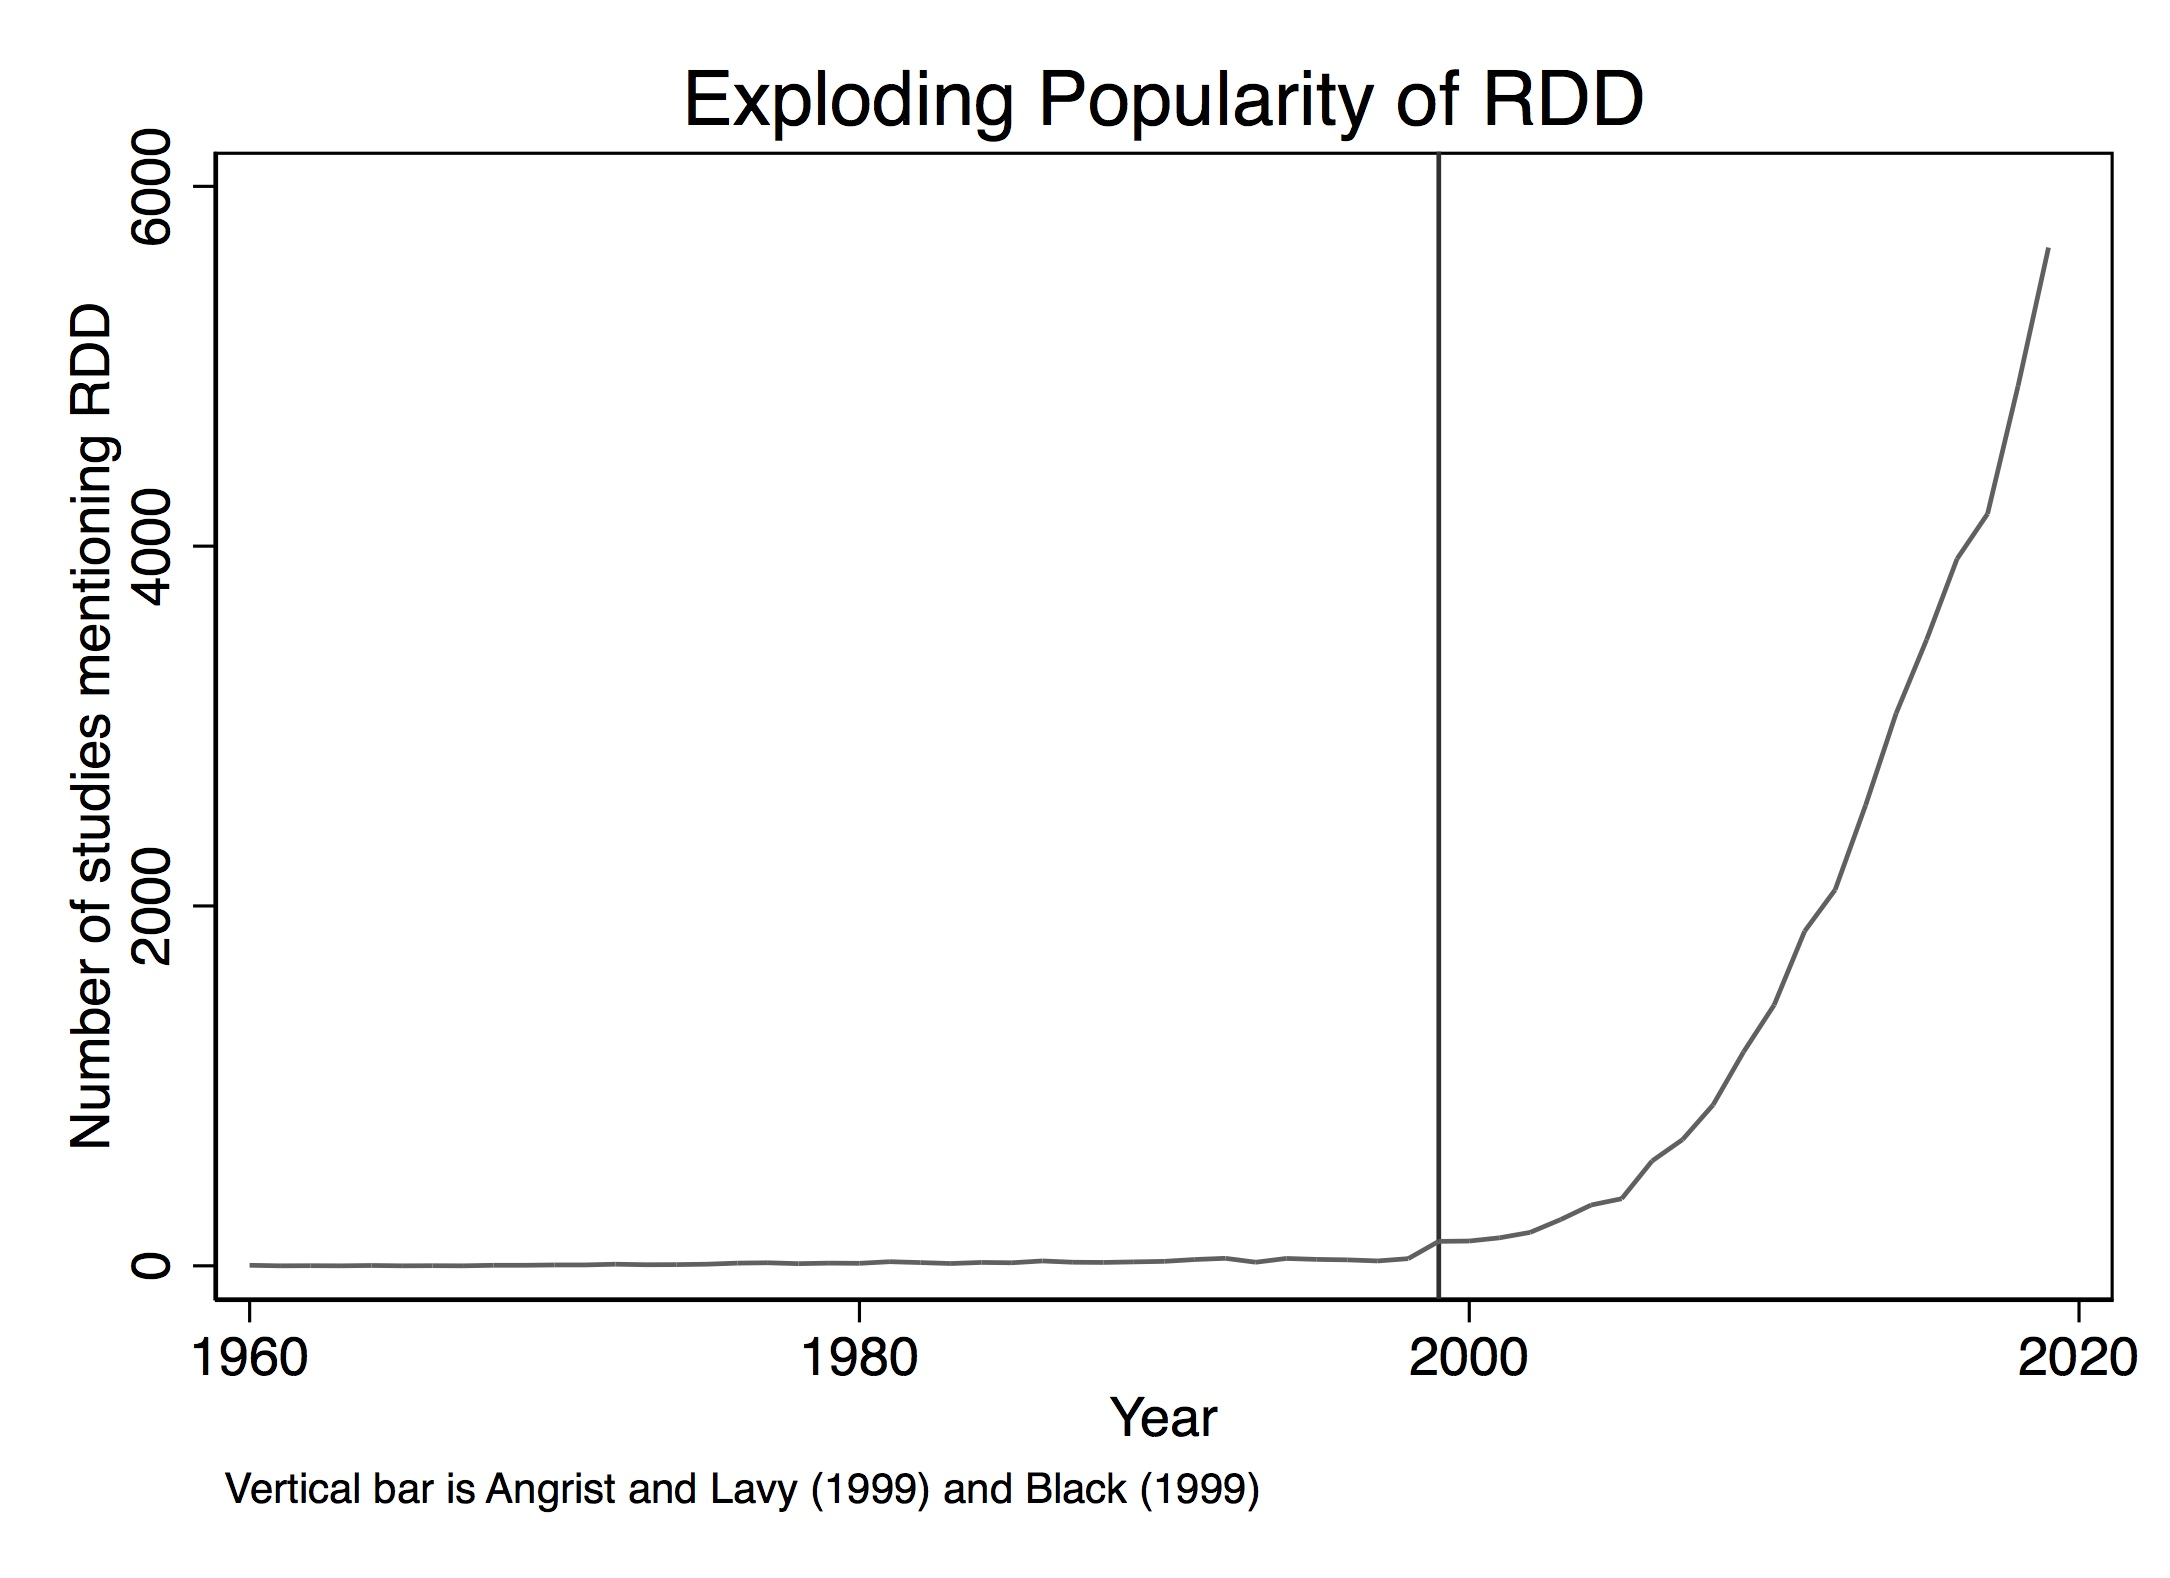
\includegraphics[scale=0.1]{img/RDD_overtime.jpg}
\end{figure}

\end{frame}

%%%%%%%%%%%%%%%%%%%%%%%%%%%%%%%%%%%%%%%%%%%%%%%%%%%%%%%%%%%%%%%%%%%%%%%%%%%%%%%%
\begin{frame}{Why the lag in adoption?}

Cook (2008): RDD was ``waiting for life to arrive''
\begin{itemize}
    \vspace{2ex}
    \item In the 1980s, economists often used models and theory to resolve issues of selection bias 
    \begin{displayquote}
    Some [economists] were taken with instrumental variable (IV) approaches that depend on discovering instruments correlated with selection but not with errors in the outcome... It was one thing to have a highly abstract, elegant and general theory about unbiased causal inference; and quite another thing for this method to generate specific applications whose causal conclusions fellow scholars saw as beyond dispute insofar as all the central assumptions were manifestly met.
    \end{displayquote}

    \vspace{3ex}
    \item \href{https://en.wikipedia.org/wiki/Credibility_revolution}{Credibility revolution in Economics}
    \begin{itemize}
        \item Acceptance of the potential outcomes framework
        \item Increased emphasis on causality
    \end{itemize}

    \vspace{3ex}
    \item Availability of large administrative datasets

\end{itemize}

\end{frame}


%%%%%%%%%%%%%%%%%%%%%%%%%%%%%%%%%%%%%%%%%%%%%%%%%%%%%%%%%%%%%%%%%%%%%%%%%%%%%%%%
\begin{frame}{Example of RDD}

\href{https://doi.org/10.1162/rest.91.4.717}{Hoekstra (2009)}: Wanted to measure the effect of attending a flagship state university on the earnings of 28 to 33 year olds
\begin{itemize}
    \item Measures the heterogeneous returns to college attendance

    \item State flagships are generally more selective than other state schools

    \item Example: Florida
    \begin{itemize}
        \item University of Florida (UF): state flagship
        \item Other public universities in Florida: University of Central Florida (UCF); University of South Florida (USF); Florida International University (FIU); Florida State University (FSU)...
    \end{itemize}
\end{itemize}

\vspace{3ex}
Example: what is the benefit of attending the state's flagship program?
\begin{itemize}
    \item Selection bias: students who selected into the flagship school may be higher ``ability;'' this results in them having higher wages than those who did not attend the flagship school
\end{itemize}


\end{frame}

%%%%%%%%%%%%%%%%%%%%%%%%%%%%%%%%%%%%%%%%%%%%%%%%%%%%%%%%%%%%%%%%%%%%%%%%%%%%%%%%
\begin{frame}{ Attending the state flagship university as a function of re-centered standardized test scores}

\begin{columns}
\begin{column}{.42\textwidth}
\begin{figure}
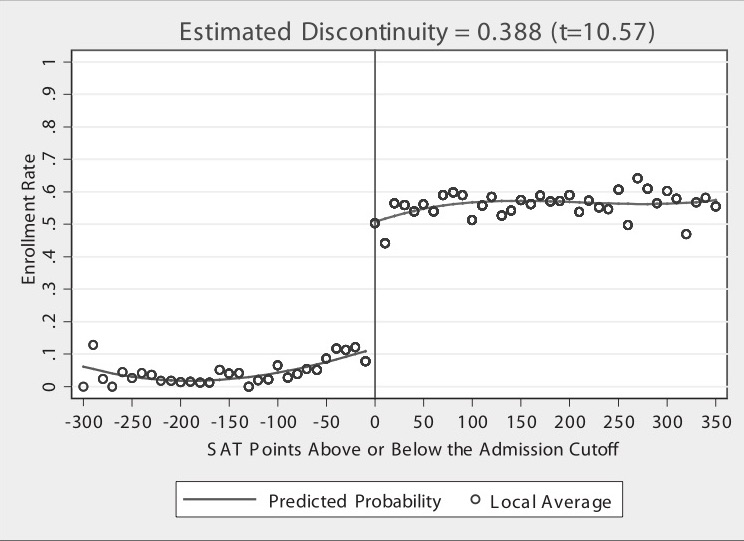
\includegraphics[scale=0.2]{img/rdd_hoekstra1.jpg}
\end{figure}
\end{column}
\begin{column}{.58\textwidth}

\begin{enumerate}
    \item Horizontal access is ``re-centered'' SAT score. The vertical line marks the cut-off (minimum SAT score for admissions)
    \begin{itemize}
        \item Re-centered SAT score is the \textbf{running variable}
    \end{itemize}

    \item Dots represent conditional mean enrollments per re-centered SAT score for many students

    \item There are two separate curvy lines. These lines are fit separately to the left and right of the cutoff

    \item There is a jump at zero in the running variable; 
    \begin{itemize}
        \item The probability of enrolling at the flagship state university jumps discontinuously when the student has the minimum SAT score required by the school
    \end{itemize}
\end{enumerate}

\end{column}
\end{columns}

% \vspace{3ex}
% \begin{itemize}
%     \item [4] There is a jump at zero in the running variable; the probability of enrolling at the flagship state university jumps discontinuously when the student has the minimum SAT score required by the school
% \end{itemize}
\end{frame}

%%%%%%%%%%%%%%%%%%%%%%%%%%%%%%%%%%%%%%%%%%%%%%%%%%%%%%%%%%%%%%%%%%%%%%%%%%%%%%%%
\begin{frame}{Interpretation of discontinuity}

Suppose the admission cut-off is 1250, 
\begin{itemize}
    \item [$\implies$] student with a 1250 has a much higher probability of attending than a student with a 1240
\end{itemize}

\vspace{3ex}
Individual student with a 1250 and individual student with a 1240 might be similar. 
\begin{itemize}
    \item Each dot in this figure represents hundreds of students
    \item Motivating assumption for RDD: how different is the average student with a 1240, and the average student with a 1250? Is there a meaningful jump in ability at that level? 
\end{itemize}


\end{frame}


% %%%%%%%%%%%%%%%%%%%%%%%%%%%%%%%%%%%%%%%%%%%%%%%%%%%%%%%%%%%%%%%%%%%%%%%%%%%%%%%%
% \begin{frame}{Estimation strategy}

% \textbf{Move to later}: FWL explanation, alongside result?
% % To measure impact of flagship school attendance on earnings, Hoekstra matches quarterly earnings records from 1998 through the second quarter of 2005 to the university records. Estimate:

% % where:
% % \begin{itemize}
% %     \item $\psi_{\text{Year}}$: time fixed effects
% %     \item $\omega_{\text{Experience}}$: years after high school 
% %     \item $\theta_{\text{Cohort}}$: cohort in which a student applied to university
% % \end{itemize}
% % Save residuals from \eqref{eq1}. Estimate RDD regression:
% % Average residual earnings is used to implement a partialled out future earnings variable according to the Frisch-Waugh-Lovell theorem. Hoekstra then takes each students’ residuals from the natural log of earnings regression and collapses them into conditional averages for bins along the recentered running variable.
% % \begin{equation}
% %     \text{Outcome} = \beta_0 + \beta_1 \cdot \mathbf{1}[\text{Above admissions cutoff}]
% %     + \beta_2
% % \end{equation}



% \end{frame}


%%%%%%%%%%%%%%%%%%%%%%%%%%%%%%%%%%%%%%%%%%%%%%%%%%%%%%%%%%%%%%%%%%%%%%%%%%%%%%%%
\begin{frame}{Estimation}

\begin{columns}
\begin{column}{.45\textwidth}
\begin{figure}
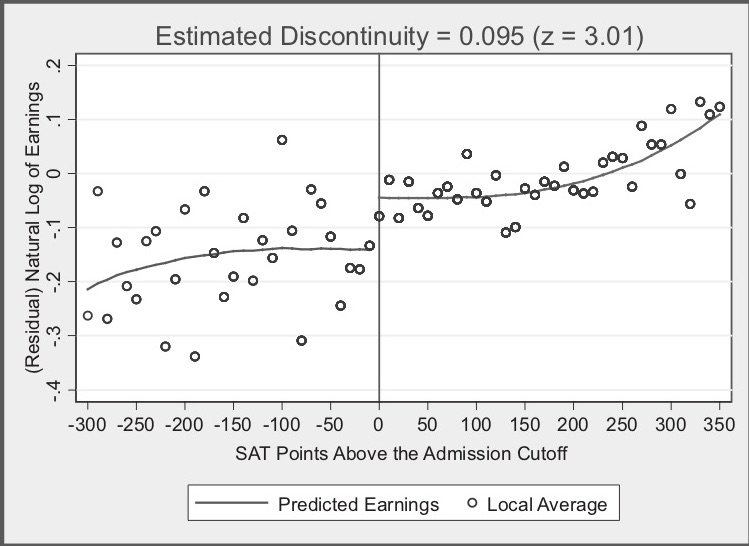
\includegraphics[scale=0.2]{img/rdd_hoekstra2.jpg}
\end{figure}
\end{column}
\begin{column}{.55\textwidth}



Impact of flagship on earnings:
\begin{itemize}
    \item Estimate individual characteristics on earnings
    \begin{equation}\label{eq1}
    \log {\text{Earnings}} = \psi_{\text{Year}} + \omega_{\text{Experience}} + \theta_{\text{Cohort}} + \epsilon
\end{equation}
Save residuals from \eqref{eq1}
    \item Average residual earnings along bins for running variable
\end{itemize}
\end{column}
\end{columns}

\end{frame}

%%%%%%%%%%%%%%%%%%%%%%%%%%%%%%%%%%%%%%%%%%%%%%%%%%%%%%%%%%%%%%%%%%%%%%%%%%%%%%%%
\begin{frame}{Interpretation of results}

``Estimated Discontinuity = 0.095 (z = 3.01)''
\begin{itemize}
    \item Those just above the cutoff earn 9.5\% higher wages in the long term than do those just below.
\end{itemize}

\vspace{3ex}
Intuitive understanding
\begin{itemize}
    \item Students with an SAT score just above the cutoff see a jump their probability of attending the state flagship
    \item Ten+ years later, these students just above the SAT cutoff see a jump in logged earnings of 9.5\%
    \item [$\implies$] Those students who barely made it into the state flagship made around 10\% more in long term earnings
\end{itemize}

\end{frame}

%%%%%%%%%%%%%%%%%%%%%%%%%%%%%%%%%%%%%%%%%%%%%%%%%%%%%%%%%%%%%%%%%%%%%%%%%%%%%%%%
\begin{frame}{Discontinuities}

RDD is about finding ``jumps'' in the probability of treatment along some running variable $X$

\vspace{3ex}
Assignment rule does not need to be arbitrary; it just needs to be known, precise, and free of manipulation. Examples:
\begin{itemize}
    \item \href{https://doi.org/10.1257/aer.20130189}{Hansen (2015):} To study the effect of harsher punishments and sanctions on driving under the influence, the authors use 0.08 BAC threshold, which increases the probability of being arrested for DWI
    \item \href{https://doi.org/10.1257/aer.98.5.2242}{Card, Dobkin, and Maestas (2008):} To study the impact of health insurance on health care utilization, the authors use the onset of Medicare eligibility at 65
    \item \href{https://doi.org/10.1162/003465304323023778}{Jacob and Lefgren (2004):} To study the effectiveness of remedial education programs like summer school, the authors use a grade threshold that increases the probability of summer school attendance 
\end{itemize}

\vspace{3ex}
In all cases: need lots of data around the discontinuities. RDD studies often use large, administrative datasets
\end{frame}

%%%%%%%%%%%%%%%%%%%%%%%%%%%%%%%%%%%%%%%%%%%%%%%%%%%%%%%%%%%%%%%%%%%%%%%%%%%%%%%%
\section[Sharp RDD]{Sharp Regression Discontinuity Design}
\miniframesoff
\begin{frame}
    \tableofcontents[currentsection]
\end{frame}
\miniframeson
%%%%%%%%%%%%%%%%%%%%%%%%%%%%%%%%%%%%%%%%%%%%%%%%%%%%%%%%%%%%%%%%%%%%%%%%%%%%%%%%


%%%%%%%%%%%%%%%%%%%%%%%%%%%%%%%%%%%%%%%%%%%%%%%%%%%%%%%%%%%%%%%%%%%%%%%%%%%%%%%%
\begin{frame}{Two types of RDD designs}


\begin{columns}
\begin{column}{.45\textwidth}
\begin{figure}
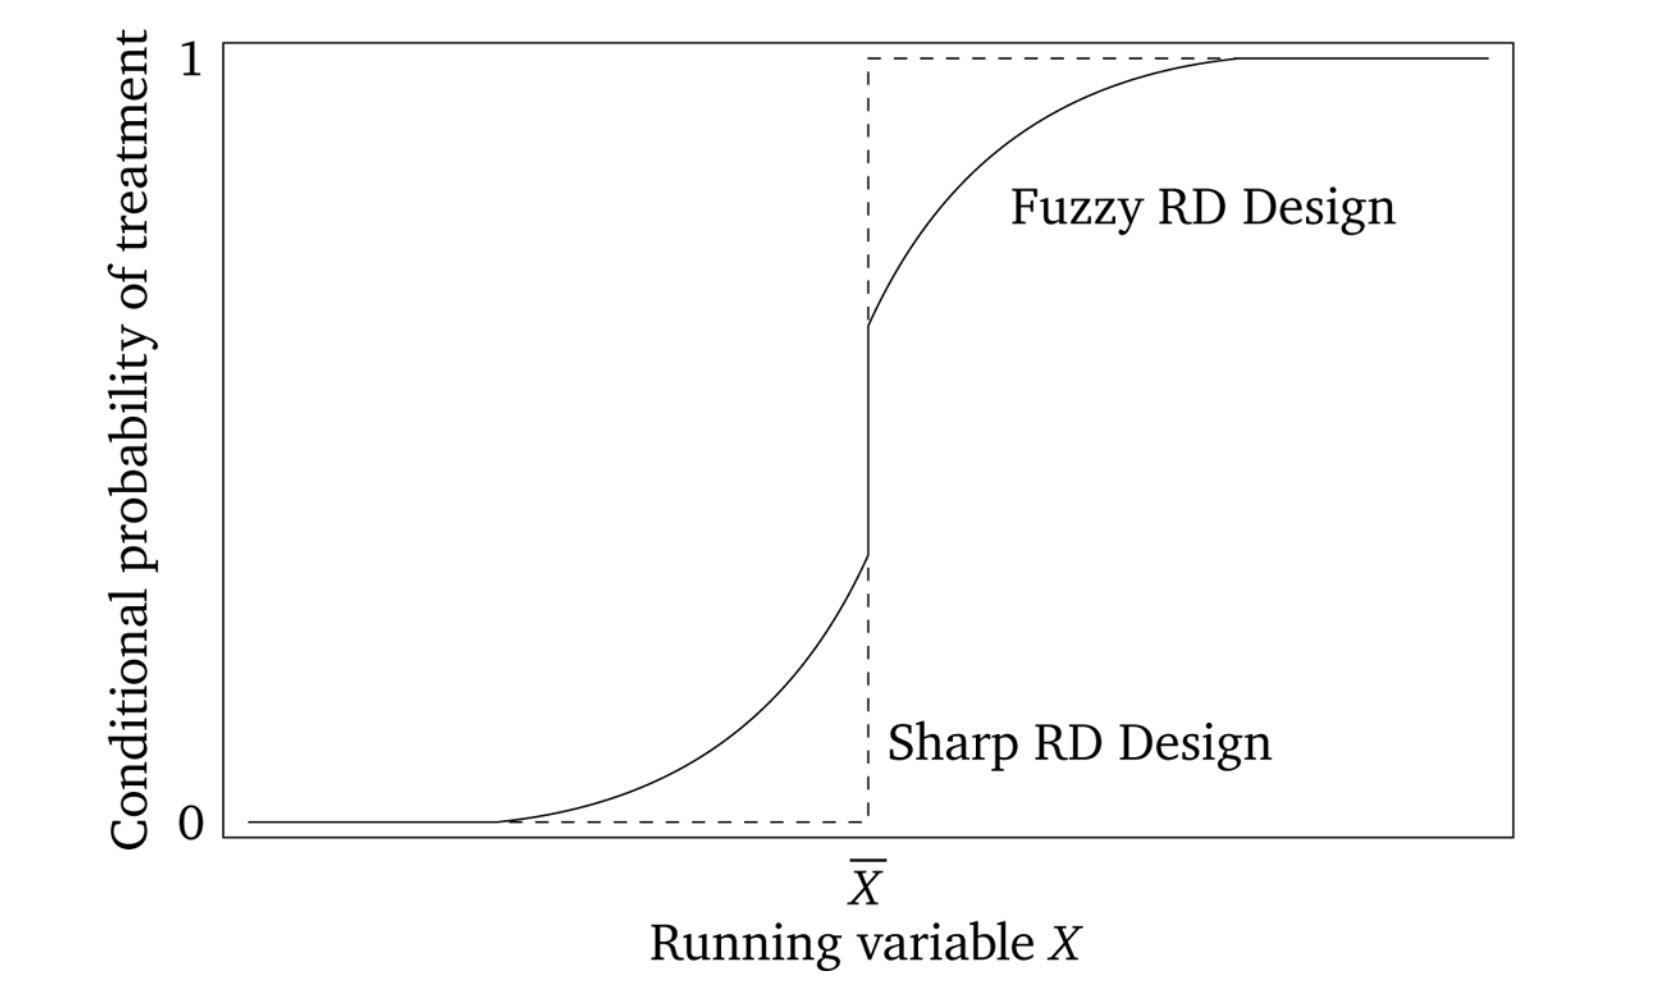
\includegraphics[scale=0.18]{img/klaauw2002.png}
\end{figure}
\end{column}
\begin{column}{.55\textwidth}

\textbf{Sharp RDD}:
\begin{itemize}
    \item Probability of treatment goes from 0 to 1 at cutoff
    \item Treatment is a \textbf{deterministic function} of running variable $X$
    \item Example: Medicare enrollment happens at 65
\end{itemize}

\vspace{3ex}
\textbf{Fuzzy RDD}:
\begin{itemize}
    \item Discontinuous ``jump'' in probability of treatment at cutoff
    \item Cutoff is used as an instrumental variable for treatment (more on this later)
\end{itemize}

\end{column}
\end{columns}
\vspace{3ex}
In both sharp and fuzzy RDD: there is some running variable $X$, where, upon reaching some cutoff $c_0$, the likelihood of treatment flips


\end{frame}

%%%%%%%%%%%%%%%%%%%%%%%%%%%%%%%%%%%%%%%%%%%%%%%%%%%%%%%%%%%%%%%%%%%%%%%%%%%%%%%%
\begin{frame}{Sharp RDD}

Treatment $D_i$ is a deterministic function of the running variable $X_i$:
\begin{equation*}
    D_i = \begin{cases} 1 &\text{ if } X_i \geq c_0 \\ 0 &\text{ if } X_i < c_0 \end{cases}
\end{equation*}
where $c_0$ is a \textbf{known} threshold or cutoff

\vspace{3ex}
Implications of sharp RDD:
\begin{itemize}
    \item If you know $X_i$, you know $D_i$
    \item There is no \textbf{overlap} along the running variable 
\end{itemize}

\end{frame}

%%%%%%%%%%%%%%%%%%%%%%%%%%%%%%%%%%%%%%%%%%%%%%%%%%%%%%%%%%%%%%%%%%%%%%%%%%%%%%%%
\begin{frame}{Potential outcomes in Sharp RDD}

Assuming constant treatment effects in sharp RDD, can write control potential outcome as:
\begin{align*}
    Y_i (0) &= \alpha + \beta X_i \\
    Y_i (1) &= Y_i (0) + \delta,
\end{align*}
where $\delta$ is the treatment effect. 

\vspace{3ex}
Can write observed $Y_i$ in terms of potential outcomes:
\begin{align*}
    Y_i &= Y_i (0) + (Y_i (1) - Y_i (0)) D_i \\
    \implies Y_i &= \alpha + \beta X_i + \delta D_i + \epsilon_i
\end{align*}
Treatment effect parameter $\delta$ is the discontinuity in the conditional expectation function:
\begin{align*}
    \delta &= \lim_{x \downarrow c_0} \EE [Y_i (1) \vert X_i = x]
    - \lim_{x \uparrow c_0} \EE [Y_i (0) \vert X_i = x]
\end{align*}

\end{frame}

%%%%%%%%%%%%%%%%%%%%%%%%%%%%%%%%%%%%%%%%%%%%%%%%%%%%%%%%%%%%%%%%%%%%%%%%%%%%%%%%
\begin{frame}{Local average treatment effect (LATE)}

Causal effect in sharp RDD at the cutoff is the \textbf{local averate treatment effect (LATE)}: 
\begin{itemize}
    \item Average causal effect as running variable approaches the cutoff in the limit
    \item Technically only identifying causal effects for those at the limit
    \item We have only estimated an average treatment effect that is \textbf{local} to the range around the cutoff
\end{itemize}
\begin{equation*}
    \delta_{SRD} = \EE [Y_i (1) - Y_i(0) \vert X_i = c_0]
\end{equation*}
In sharp RDD, \textbf{extrapolation} plays an important role
\begin{itemize}
    \item There is no overlap in treatment before and after the cut-off
\end{itemize}
\textbf{Notebook: } generate simulated data


\end{frame}

%%%%%%%%%%%%%%%%%%%%%%%%%%%%%%%%%%%%%%%%%%%%%%%%%%%%%%%%%%%%%%%%%%%%%%%%%%%%%%%%
\begin{frame}{Continuity assumption}

Key assumption in Sharp RDD: continuitiy of potential outcomes
\begin{itemize}
    \item $\EE [Y_0 \vert X = c_0]$ and $\EE [Y_1 \vert X = c_0]$ are \textbf{continuous functions} of $X$, even across the threshold $c_0$
    \item Absent treatment, potential outcomes wouldn't have jumped
    \item \textbf{Fundamentally untestable assumption}
\end{itemize}

\vspace{3ex}
Example: \href{https://doi.org/10.1257/app.1.1.164}{Carpenter and Dobkin (2009)}
\begin{itemize}
    \item Effect of alcohol consumption on mortality (specifically car crashes)
    \item If there's a discontinuous jump in drinking at 21, and that causes more people to drive drunk, that may  result in more deaths from motor vehical accidents (MVAs)
    \item Continuity assumption: nothing else could happen that causes mortality of 21 year olds to jump
\end{itemize}
\end{frame}

%%%%%%%%%%%%%%%%%%%%%%%%%%%%%%%%%%%%%%%%%%%%%%%%%%%%%%%%%%%%%%%%%%%%%%%%%%%%%%%%
\begin{frame}{Continuity assumption: example}

% \begin{columns}
% \begin{column}{.4\textwidth}
% \begin{figure}
% 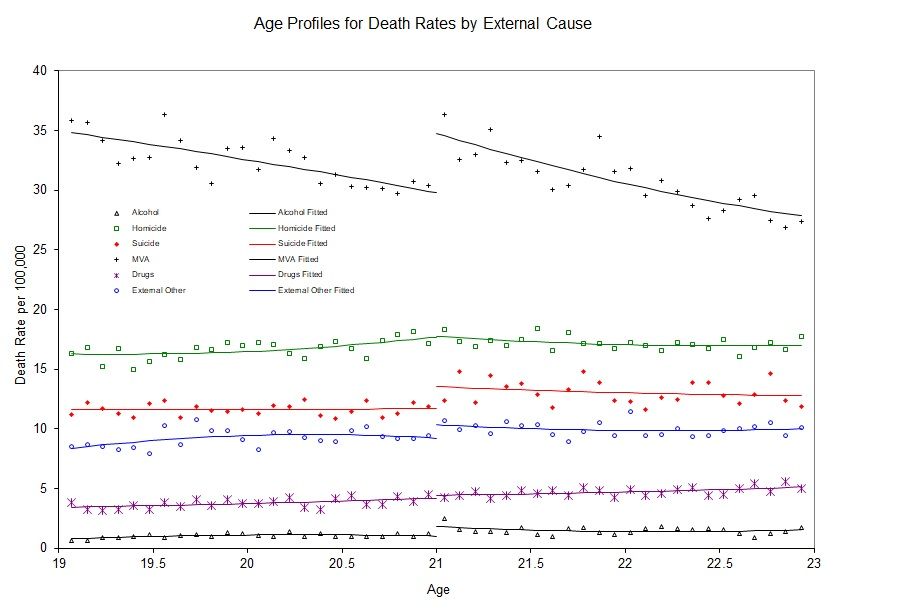
\includegraphics[scale=0.3]{img/carpenter1.jpg}
% \end{figure}
% \end{column}

% \begin{column}{.6\textwidth}
% \begin{itemize}
%     \item There is a discontinuous jump in motor vehicle deaths at 21
%     \item Most likely explanation is that age 21 causes people to drink more, and sometimes even while they are driving 
%     \item This is only a causal effect if motor vehicle accidents don’t jump at age 21 for other reason
% \end{itemize}
% \end{column}
% \end{columns}

\begin{figure}
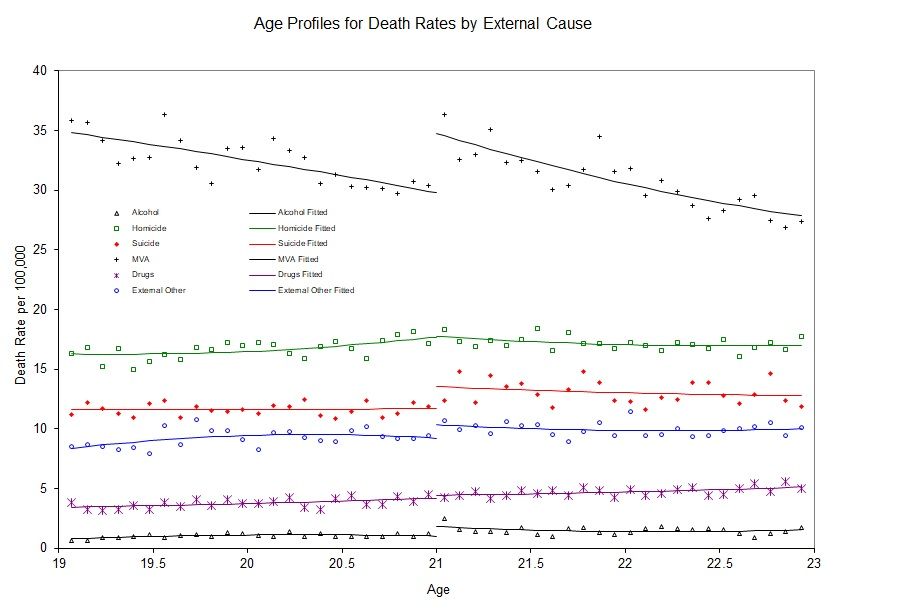
\includegraphics[scale=0.3]{img/carpenter1.jpg}
\end{figure}

\begin{itemize}
    \item There is a discontinuous jump in motor vehicle deaths at 21
    \item Most likely explanation is that age 21 causes people to drink more, and sometimes even while they are driving 
    \item This is only a causal effect if motor vehicle accidents don’t jump at age 21 for other reason
\end{itemize}
\textbf{Example notebook}

\end{frame}

%%%%%%%%%%%%%%%%%%%%%%%%%%%%%%%%%%%%%%%%%%%%%%%%%%%%%%%%%%%%%%%%%%%%%%%%%%%%%%%%
\section[Sharp RDD Estimation]{Sharp Regression Discontinuity Design Estimation}
\miniframesoff
\begin{frame}
    \tableofcontents[currentsection]
\end{frame}
\miniframeson
%%%%%%%%%%%%%%%%%%%%%%%%%%%%%%%%%%%%%%%%%%%%%%%%%%%%%%%%%%%%%%%%%%%%%%%%%%%%%%%%

%!TEX root = ./slides-09-rd.tex
%%%%%%%%%%%%%%%%%%%%%%%%%%%%%%%%%%%%%%%%%%%%%%%%%%%%%%%%%%%%%%%%%%%%%%%%%%%%%%%%
\begin{frame}{Centering running variable}

Common for authors to ``re-center'' running variable $X_i$ by subtracting the cut-off, $c_0$. 

\begin{align*}
    Y_i &= \beta_0 + \beta_1 X_i + \delta D_i + \epsilon_i \\
    \implies Y_i &= \beta_0 + \beta_1 (X_i - c_0) + \delta D_i + \epsilon_i \\
    =& (\beta_0 - \beta_1 \cdot c_0) + \beta_1 X_i + \delta D_i + \epsilon_i \\
    =& \alpha + \beta_1 X_i + \delta D_i + \epsilon_i
\end{align*}
Variables can maintain the same interpretation if we re-center the running variable $X_i$ and change the intercept


\end{frame}

%%%%%%%%%%%%%%%%%%%%%%%%%%%%%%%%%%%%%%%%%%%%%%%%%%%%%%%%%%%%%%%%%%%%%%%%%%%%%%%%
\begin{frame}{Linear Sharp RDD}

\textbf{Goal: } estimate treatment effect at the cut-off, $c_0$


\begin{itemize}
    \item Many sharp RDDs are nonlinear, but it's helpful to start thinking about estimation in a linear model:
\end{itemize}
\begin{equation*}
    Y_i = \beta_0 + \beta_1 X_i + \beta_2 \mathbf{1}\{X_i > c_0\} +  \beta_3  \mathbf{1}\{X_i > c_0\} X_i
\end{equation*}
\begin{itemize}
    \item Estimating this equation is the same as estimating a linear model above and below the threshold
    \begin{itemize}
        \item $\beta_0$ is intercept before cut-off
        \item $\beta_0 + \beta_2$ is intercept after cut-off
    \end{itemize}
\end{itemize}
Why do we re-center the running variable $X_i$?
\begin{itemize}
    \item If you re-center the model, $\beta_0$ is the predicted value at the threshold, for the values below $c_0$
    \begin{equation*}
        \beta_0 = \lim_{x \uparrow c} \EE [Y \vert X_i = x]
    \end{equation*}
    \item Then $\beta_0 + \beta_2$ is the predicted value at the threshold, for values above $c_0$
    \begin{equation*}
        \beta_0 + \beta_2 = \lim_{x \downarrow c} \EE [Y \vert X_i = x]
    \end{equation*}
\end{itemize}
$\implies$ ATE equals $\beta_2$

\end{frame}



%%%%%%%%%%%%%%%%%%%%%%%%%%%%%%%%%%%%%%%%%%%%%%%%%%%%%%%%%%%%%%%%%%%%%%%%%%%%%%%%
\begin{frame}{Nonlinearities}

\begin{columns}
\begin{column}{.5\textwidth}
\begin{figure}
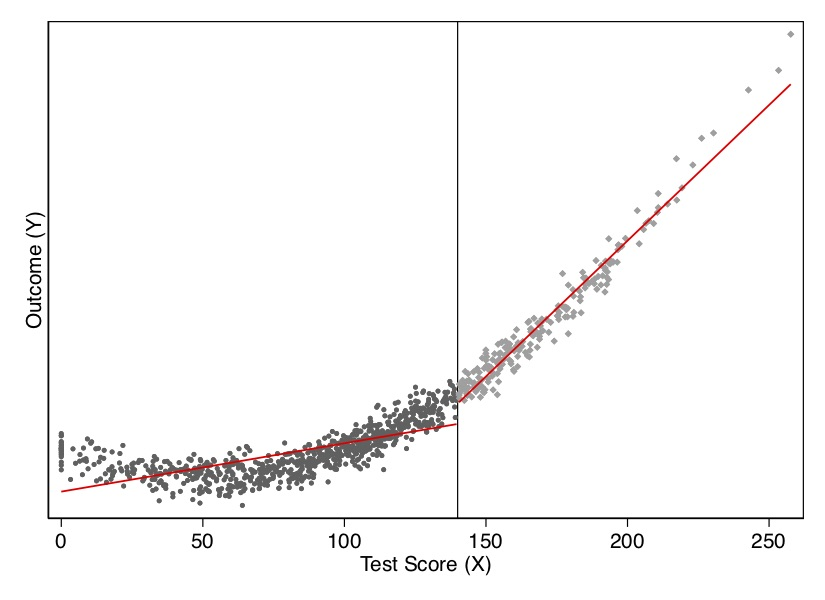
\includegraphics[scale=0.2]{img/rdd_simul4.jpg}
\end{figure}
\end{column}
\begin{column}{.5\textwidth}
\begin{itemize}
    \item True data generating process is nonlinear
    \item Using a linear model may lead to a spurious example
    \item On the left: fitting a model using a least squares regression controlling for the running variable estimates a causal effect though there isn’t one
\end{itemize}
\end{column}
\end{columns}

\end{frame}

%%%%%%%%%%%%%%%%%%%%%%%%%%%%%%%%%%%%%%%%%%%%%%%%%%%%%%%%%%%%%%%%%%%%%%%%%%%%%%%%
\begin{frame}{Nonlinearities}

Suppose the nonlinear relationship is:
\begin{equation*}
    \EE [Y_i (0) \vert X_i] = f(X_i),
\end{equation*}
where $f (X_i)$ is a reasonably smooth function of $X_i$. Then fit the regression model:
\begin{equation*}
    Y_i = f(X_i) + \delta D_i + \epsilon_i
\end{equation*}
Question: since $f(X_i)$ is unobservable for $X_i > c_0$, how do you model the nonlinearity?
\begin{enumerate}
    \item Estimate $f(X_i)$ using a $p$-th order polynomial
    \item Nonparametric kernel estimation
\end{enumerate}


\end{frame}

%%%%%%%%%%%%%%%%%%%%%%%%%%%%%%%%%%%%%%%%%%%%%%%%%%%%%%%%%%%%%%%%%%%%%%%%%%%%%%%%
\begin{frame}{Nonlinear estimation: polynomial}

Generate $f(X_i)$ by allowing $X_i$ to differ on both sides of the cutoff. Letting $\tilde{X}_i$ be the centered running variable:
\begin{align*}
    \EE [Y_i (0) \vert X_i] &= \alpha + \beta_{01} \tilde{X}_i + \beta_{02} \tilde{X}_i^2 + \dots + \beta_{0p} \tilde{X}_i^p \\
    \EE [Y_i (1) \vert X_i] &= \alpha + \delta + \beta_{11} \tilde{X}_i + \beta_{12} \tilde{X}_i^2 + \dots + \beta_{1p} \tilde{X}_i^p \\
\end{align*}
Translating this into observed $Y_i$:
\begin{align*}
    \EE [Y_i \vert X_i] &= 
    \EE [Y_i (0) \vert X_i] + \Big( \EE [Y_i (1) \vert X_i] - \EE [Y_i (0) \vert X_i] \Big) D_i 
\end{align*}
Regression model given by:
\begin{equation*}
    Y_i = \alpha + \beta_{01} \tilde{X}_i + \beta_{02} \tilde{X}_i^2 + \dots + \beta_{0p} \tilde{X}_i^p
    + \delta D_i
    + \beta_{1}^* D_i \tilde{X}_i + \beta_{2}^* D_i \tilde{X}_i^2 + \dots + \beta_{p}^* D_i \tilde{X}_i^p + \epsilon_i
\end{equation*}
where $\beta_{p}^* = \beta_{1p} - \beta_{0p}$. 
\begin{itemize}
    \item At $c_0$, treatment effect given by $\delta$
    \item At $c > c_0$, treatment effect given by $\delta + \beta_1^* c + \beta_2^* c^2 + \dots + \beta_p^* c^p$
    % \item At $X_i > c_0$, treatment effect given by $\delta + \beta_1^* c$
\end{itemize}

\end{frame}

%%%%%%%%%%%%%%%%%%%%%%%%%%%%%%%%%%%%%%%%%%%%%%%%%%%%%%%%%%%%%%%%%%%%%%%%%%%%%%%%
\begin{frame}{Nonlinear estimation: polynomial}


Validity of RDD estimates using polynomials depends on whether polynomial model provides an accurdate description of $\EE[Y_i (0) \vert X_i]$
\begin{itemize}
    \item If polynomial model is not appropriate, then what looks like a jump might actually just be unaccounted for nonlinearity
\end{itemize}

\vspace{3ex}
\href{https://doi.org/10.1080/07350015.2017.1366909}{Gelman and Imbens (2019)}: ``Why High-Order Polynomials Should Not Be Used in Regression Discontinuity Designs''
\begin{itemize}
    \item Controlling for higher-order polynomials (3+) can lead to nonsensical results
    \item Three major problems: 
    \begin{itemize}
        \item Noisy estimates
        \item Sensitivity to degree of the polynomial
        \item Poor coverage of confidence intervals
    \end{itemize}
    \item Authors recommend local linear or quadratic polynomials or other smooth functions
\end{itemize}

\vspace{3ex}
That said, it's conceptually important, and used in older papers!
% so we'll review it: \textbf{Example notebook}

\end{frame}

%%%%%%%%%%%%%%%%%%%%%%%%%%%%%%%%%%%%%%%%%%%%%%%%%%%%%%%%%%%%%%%%%%%%%%%%%%%%%%%%
\begin{frame}{Nonlinear estimation: kernel estimation}

Kernel regression provides an alternative to using higher-order polynomials

\vspace{3ex}
Regression Discontinuity relies heavily on the extrapolation 
\begin{itemize}
    \item Looking at the values at the beginning and end of 2 regression lines
    \item If regression is focusing on fitting other data points, rather than correctly fitting at the threshold, the treatment effect might be misspecified
\end{itemize}

\vspace{3ex}
\textbf{Possible solution:} give higher weights to points close to the cutoff $c_0$

\vspace{3ex}
\href{https://doi.org/10.1111/1468-0262.00183}{Hahn, Todd, and Van der Klaauw (2001)}: 
\begin{itemize}
    \item To avoid poor boundary performance, use weighted regression restricted to a window (``local'') 
    % \item Local linear estimators have better boundary properties than the traditional kernel regression estimat 
    \item In local kernel regression: ``kernel'' provides weights close to the cut-off; can then use weighted least squares to estimate effects
\end{itemize}


\end{frame}



%%%%%%%%%%%%%%%%%%%%%%%%%%%%%%%%%%%%%%%%%%%%%%%%%%%%%%%%%%%%%%%%%%%%%%%%%%%%%%%%
\begin{frame}{Kernel weighting function}

Re-weight sample using the \textbf{triangle kernel}:
\begin{equation*}
    K (X, c_0, h) = \mathbf{1} \{ \vert X - c_0 \vert \leq h\} \cdot \left( 1 - \frac{X - c_0}{h} \right)
\end{equation*}
\begin{itemize}
    \item $\vert X - c_0 \vert \leq h$: The absolute difference between $X$ and $c_0$ is less than or equal to some \textbf{bandwidth} $h$
    \item $\mathbf{1} \{ \vert X - c_0 \vert \leq h\}$: Indicator function that equals 1 if X is sufficiently close to $c_0$, according to the bandwidth $h$; 0 otherwise
    \item $\left( 1 - \frac{X - c_0}{h} \right)$: re-weighting function
    \begin{itemize}
        \item Ignore cases where $X - c_0 > h$, because of the indicator function
        \item We know $(X - c_0) / h$ is less than or equal to 1
        \item The further $X$ is from $c$, the larger this fraction is
        \item Because this fraction is subtracted from 1, the weights get smaller the farter $X$ is from the cut-off
    \end{itemize}
\end{itemize}



\end{frame}


%%%%%%%%%%%%%%%%%%%%%%%%%%%%%%%%%%%%%%%%%%%%%%%%%%%%%%%%%%%%%%%%%%%%%%%%%%%%%%%%
\begin{frame}{Kernel regression}

Once you've established kernel weighting function, you can use \textbf{weighted least squares} to estimate regression

\begin{equation*}
    (a, b) = \arg \min_{a, b} \sum_{i=1}^n \left(Y_i - a - b (X_i - c_0) \right)^2 K (X, c_0, h)
\end{equation*}

Note: 
\begin{itemize}
    \item This method is sensitive to the choice of bandwidth $h$. There is a lot of work out there about determining the proper bandwidth!
\end{itemize}


\end{frame}

% %%%%%%%%%%%%%%%%%%%%%%%%%%%%%%%%%%%%%%%%%%%%%%%%%%%%%%%%%%%%%%%%%%%%%%%%%%%%%%%%
% \begin{frame}{}

% \textbf{Possible to do:}
% \begin{itemize}
%     \item 6.2.5 on Medicare example
%     \item 6.2.6. on inference (standard errors)
%     \item Link to notebook going through website example
% \end{itemize}

% \end{frame}


%%%%%%%%%%%%%%%%%%%%%%%%%%%%%%%%%%%%%%%%%%%%%%%%%%%%%%%%%%%%%%%%%%%%%%%%%%%%%%%%
\section[Fuzzy RDD]{Fuzzy Regression Discontinuity Design}
\miniframesoff
\begin{frame}
    \tableofcontents[currentsection]
\end{frame}
\miniframeson
%%%%%%%%%%%%%%%%%%%%%%%%%%%%%%%%%%%%%%%%%%%%%%%%%%%%%%%%%%%%%%%%%%%%%%%%%%%%%%%%

%%%%%%%%%%%%%%%%%%%%%%%%%%%%%%%%%%%%%%%%%%%%%%%%%%%%%%%%%%%%%%%%%%%%%%%%%%%%%%%%
\begin{frame}{Fuzzy RDD}

Sharp RDD: treatment determined when $X_i \geq c_0$

\vspace{3ex}
Sometimes discontinuity is not deterministic
\begin{itemize}
    \item Fuzzy RDD: increase in the probability of treatment assignment 
    \item May happen if incentives change at some threshold, which may move some, but not all, observations to treated
\end{itemize}

\vspace{3ex}
In terms of limits:
\begin{equation*}
    \lim_{X_i \rightarrow c_0} \PP (D_i = 1 \vert X_i = c_0) \neq 
    \lim_{c_0 \leftarrow X_i} \PP (D_i = 1 \vert X_i = c_0)
\end{equation*}{}



\end{frame}


%%%%%%%%%%%%%%%%%%%%%%%%%%%%%%%%%%%%%%%%%%%%%%%%%%%%%%%%%%%%%%%%%%%%%%%%%%%%%%%%
\begin{frame}{Fuzzy RD: Continuity assumption}

\begin{columns}
\begin{column}{.4\textwidth}
\begin{figure}
\caption{Observed data in Fuzzy RDD}
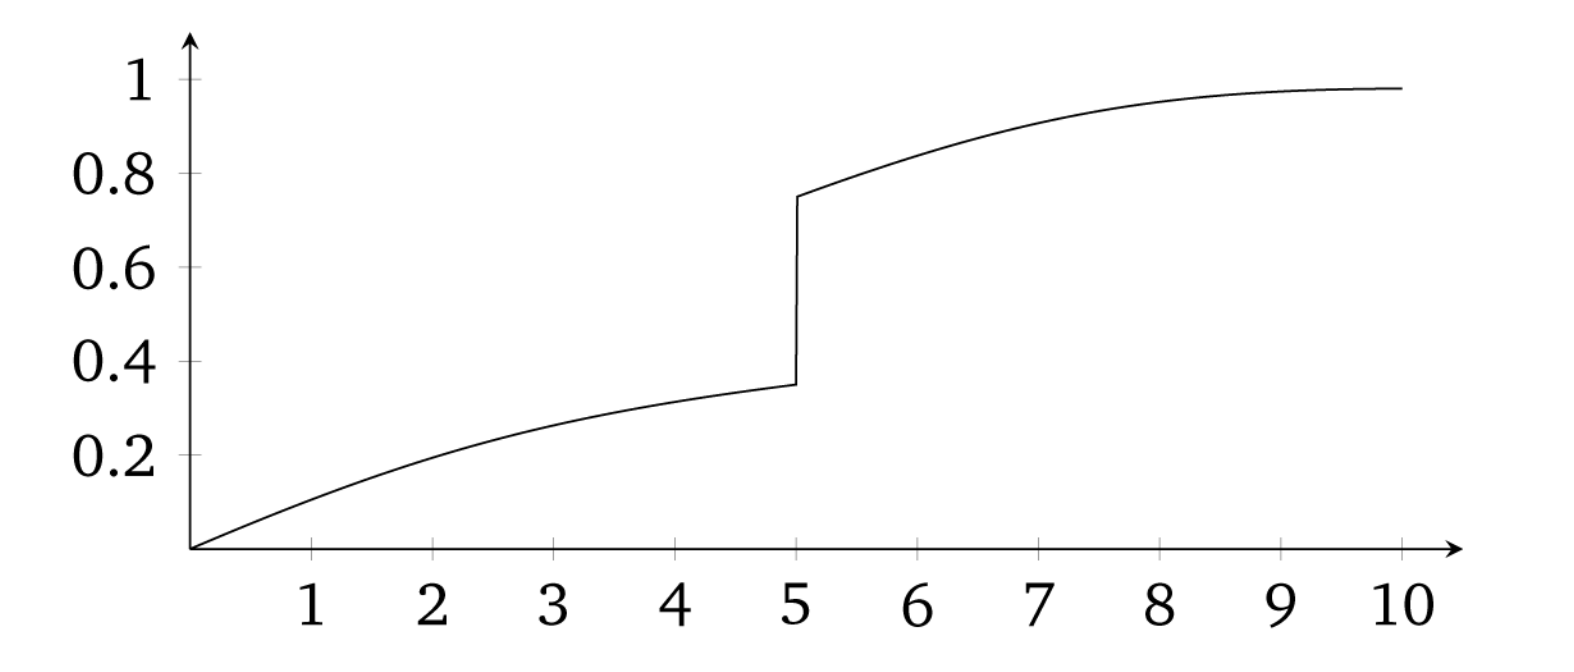
\includegraphics[scale=0.2]{img/fuzzy1.png}
\end{figure}
\begin{figure}
\caption{Continuity assumption in Fuzzy RDD}
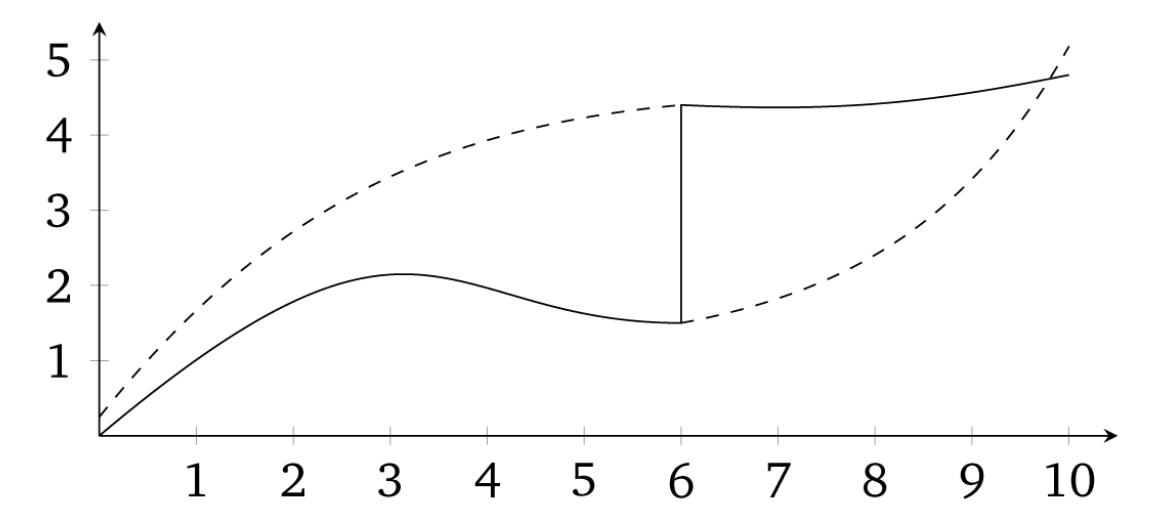
\includegraphics[scale=0.25]{img/fuzzy2.png}
\end{figure}
\end{column}

\begin{column}{.5\textwidth}
\href{https://www.sciencedirect.com/science/article/abs/pii/S0304407607001091}{Imbens and Lemieux (2008)}
\begin{itemize}
    \item Assume the conditional expectation of potential outcomes is smooth throughout the cutoff $c_0$
    \item What changes at $c_0$ is the treatment assignment probability
\end{itemize}

\end{column}

\end{columns}

\end{frame}

%%%%%%%%%%%%%%%%%%%%%%%%%%%%%%%%%%%%%%%%%%%%%%%%%%%%%%%%%%%%%%%%%%%%%%%%%%%%%%%%
\begin{frame}{Fuzzy RDD: Estimation}

Can estimate effects using a type of Wald estimator:
\begin{equation*}
    \delta_{\text{Fuzzy RDD}}
    = \frac{
        \lim_{x \downarrow c_0 \EE [Y \vert X = x]} - \lim_{x \uparrow c_0} \EE [Y \vert X = x]
        }{
            \lim_{x \downarrow c_0 \EE [D \vert X = x]} - \lim_{x \uparrow c_0} \EE [D \vert X = x]
        }
    % \frac{}{}
\end{equation*}

Fuzzy designs are numerically equivalent and conceptually similar to IV:
\begin{itemize}
    \item ``Reduced form'' numerator: ``jump'' in regression of the outcome on the running variable $X$
    % \item %(check for weak instruments using F test on instrument in first stage)
\end{itemize}

Similar IV assumptions that we will discuss in the next section 
\begin{itemize}
    \item Monotonicity: $X$ crossing a threshold cannot simultaneously cause some units to take up and others to reject $D$
    \item Excludability: $X$ crossing the cutoff cannot impact $Y$ except through impacting the receipt of $D$
\end{itemize}
Under these assumptions:
\begin{equation*}
    \delta_{\text{Fuzzy RDD}} = \EE [Y_i (1) - Y_i (0) \vert T = c, X=c]
\end{equation*}
$T=c$ are units that receive treatment when $X > c$, but not otherwise. 
\begin{itemize}
    \item This is a \textbf{local ATE (LATE)}; an effect for a subpopulation locally at $X=c_0$
\end{itemize}

\end{frame}

%%%%%%%%%%%%%%%%%%%%%%%%%%%%%%%%%%%%%%%%%%%%%%%%%%%%%%%%%%%%%%%%%%%%%%%%%%%%%%%%
\section[Challenges]{Challenges}
\miniframesoff
\begin{frame}
    \tableofcontents[currentsection]
\end{frame}
\miniframeson
%%%%%%%%%%%%%%%%%%%%%%%%%%%%%%%%%%%%%%%%%%%%%%%%%%%%%%%%%%%%%%%%%%%%%%%%%%%%%%%%

%%%%%%%%%%%%%%%%%%%%%%%%%%%%%%%%%%%%%%%%%%%%%%%%%%%%%%%%%%%%%%%%%%%%%%%%%%%%%%%%
\begin{frame}{Challenges to RDD}

Continuity assumption required for RDD. This assumption may not hold if:
\begin{itemize}
    \item Manipulation on the running variable
    \item Endogeneity of the cutoff
\end{itemize}
Most robustness is aimed at building credibility around these

\end{frame}


%%%%%%%%%%%%%%%%%%%%%%%%%%%%%%%%%%%%%%%%%%%%%%%%%%%%%%%%%%%%%%%%%%%%%%%%%%%%%%%%
\begin{frame}{Manipulating running variable}

Treatment is not as good as randomly assigned around the cutoff, $c_0$, when agents are able to manipulate their running variable scores. This happens when:
\begin{enumerate}
      \item The assignment rule is known in advance
      \item Agents are interested in adjusting
      \item Agents have time to adjust
      \item Administrative quirks like nonrandom heaping along the running
  \end{enumerate}  

\vspace{3ex}
$\implies$ Looking for evidence that people are \emph{choosing} their $X_i$ values, so as to barely receive/avoid treatment
\begin{itemize}
    \item If people who sort along their running variable have different potential outcomes, your treatment effect estimation may be biased
    \item Testable implication: if there's no manipulation, then the density of $X$ should be smooth around the cutoff
\end{itemize}

\end{frame}

%%%%%%%%%%%%%%%%%%%%%%%%%%%%%%%%%%%%%%%%%%%%%%%%%%%%%%%%%%%%%%%%%%%%%%%%%%%%%%%%
\begin{frame}{McCrary Density Test}

Null hypothesis: density is continuous at the cutoff point
\begin{itemize}
    \item Alternative hypothesis: the density increases at the cutoff (may happen if the treatment is desirable)
\end{itemize}
Method:
\begin{itemize}
    \item Count observations for a chosen bin (needs multiple units in other
words per bin)
\item Estimate nonlinear OLS model with quadratics in the running
variable on the counts
\item If unable to reject the null, that's a sign of manipulation
\end{itemize}

% This is oftentimes visualized with confidence intervals illustrating the
% effect of the discontinuity on density - you need no jump to pass this
% test
% Not perfect, but pretty ingenious and is based on rational choice
% when you think about it
Simulated data:
\begin{figure}
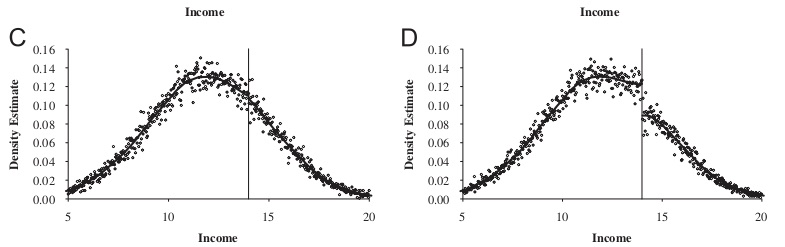
\includegraphics[scale=0.2]{img/mccrary_density_test.jpg}
\end{figure}

\end{frame}

%%%%%%%%%%%%%%%%%%%%%%%%%%%%%%%%%%%%%%%%%%%%%%%%%%%%%%%%%%%%%%%%%%%%%%%%%%%%%%%%
\begin{frame}{Placebo tests}

For continuity assumption to hold, the only thing that causes the outcome to change abruptly at the cutoff is the treatment.
\begin{itemize}
    \item [$\implies$] There should not be discontinuous changes in average values of reasonably chosen covariates around the cutoff
\end{itemize}

\vspace{2ex} \textbf{Placebo test:}
\begin{itemize}
    \item If your continuity assumption is reasonable, Make sure there is no effect around reasonable chosen pre-treatment variables
\end{itemize}

\begin{figure}
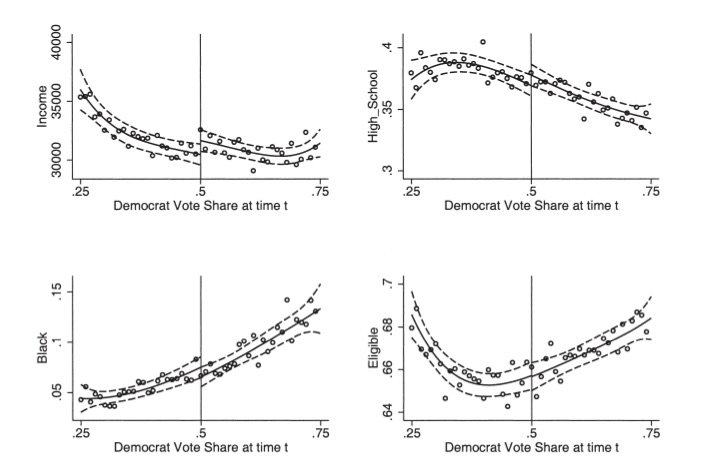
\includegraphics[scale=0.23]{img/lee_moretti_butler_fig3.jpg}
\end{figure}

\end{frame}


%%%%%%%%%%%%%%%%%%%%%%%%%%%%%%%%%%%%%%%%%%%%%%%%%%%%%%%%%%%%%%%%%%%%%%%%%%%%%%%%
\begin{frame}{Heaping}

What is the causal effect of heightened medical care for premature
babies on infant mortality?
\begin{itemize}
    \item Babies with very low birth weights ($<1500$g) are automatically admitted to the NICU
\end{itemize}
Problem with using this cutoff: heaping
\begin{itemize}
    \item Unlikely babies are naturally born at intervals of 100g
    \item Likely that there is some manipulation of running variable $X$
\end{itemize}


\begin{figure}
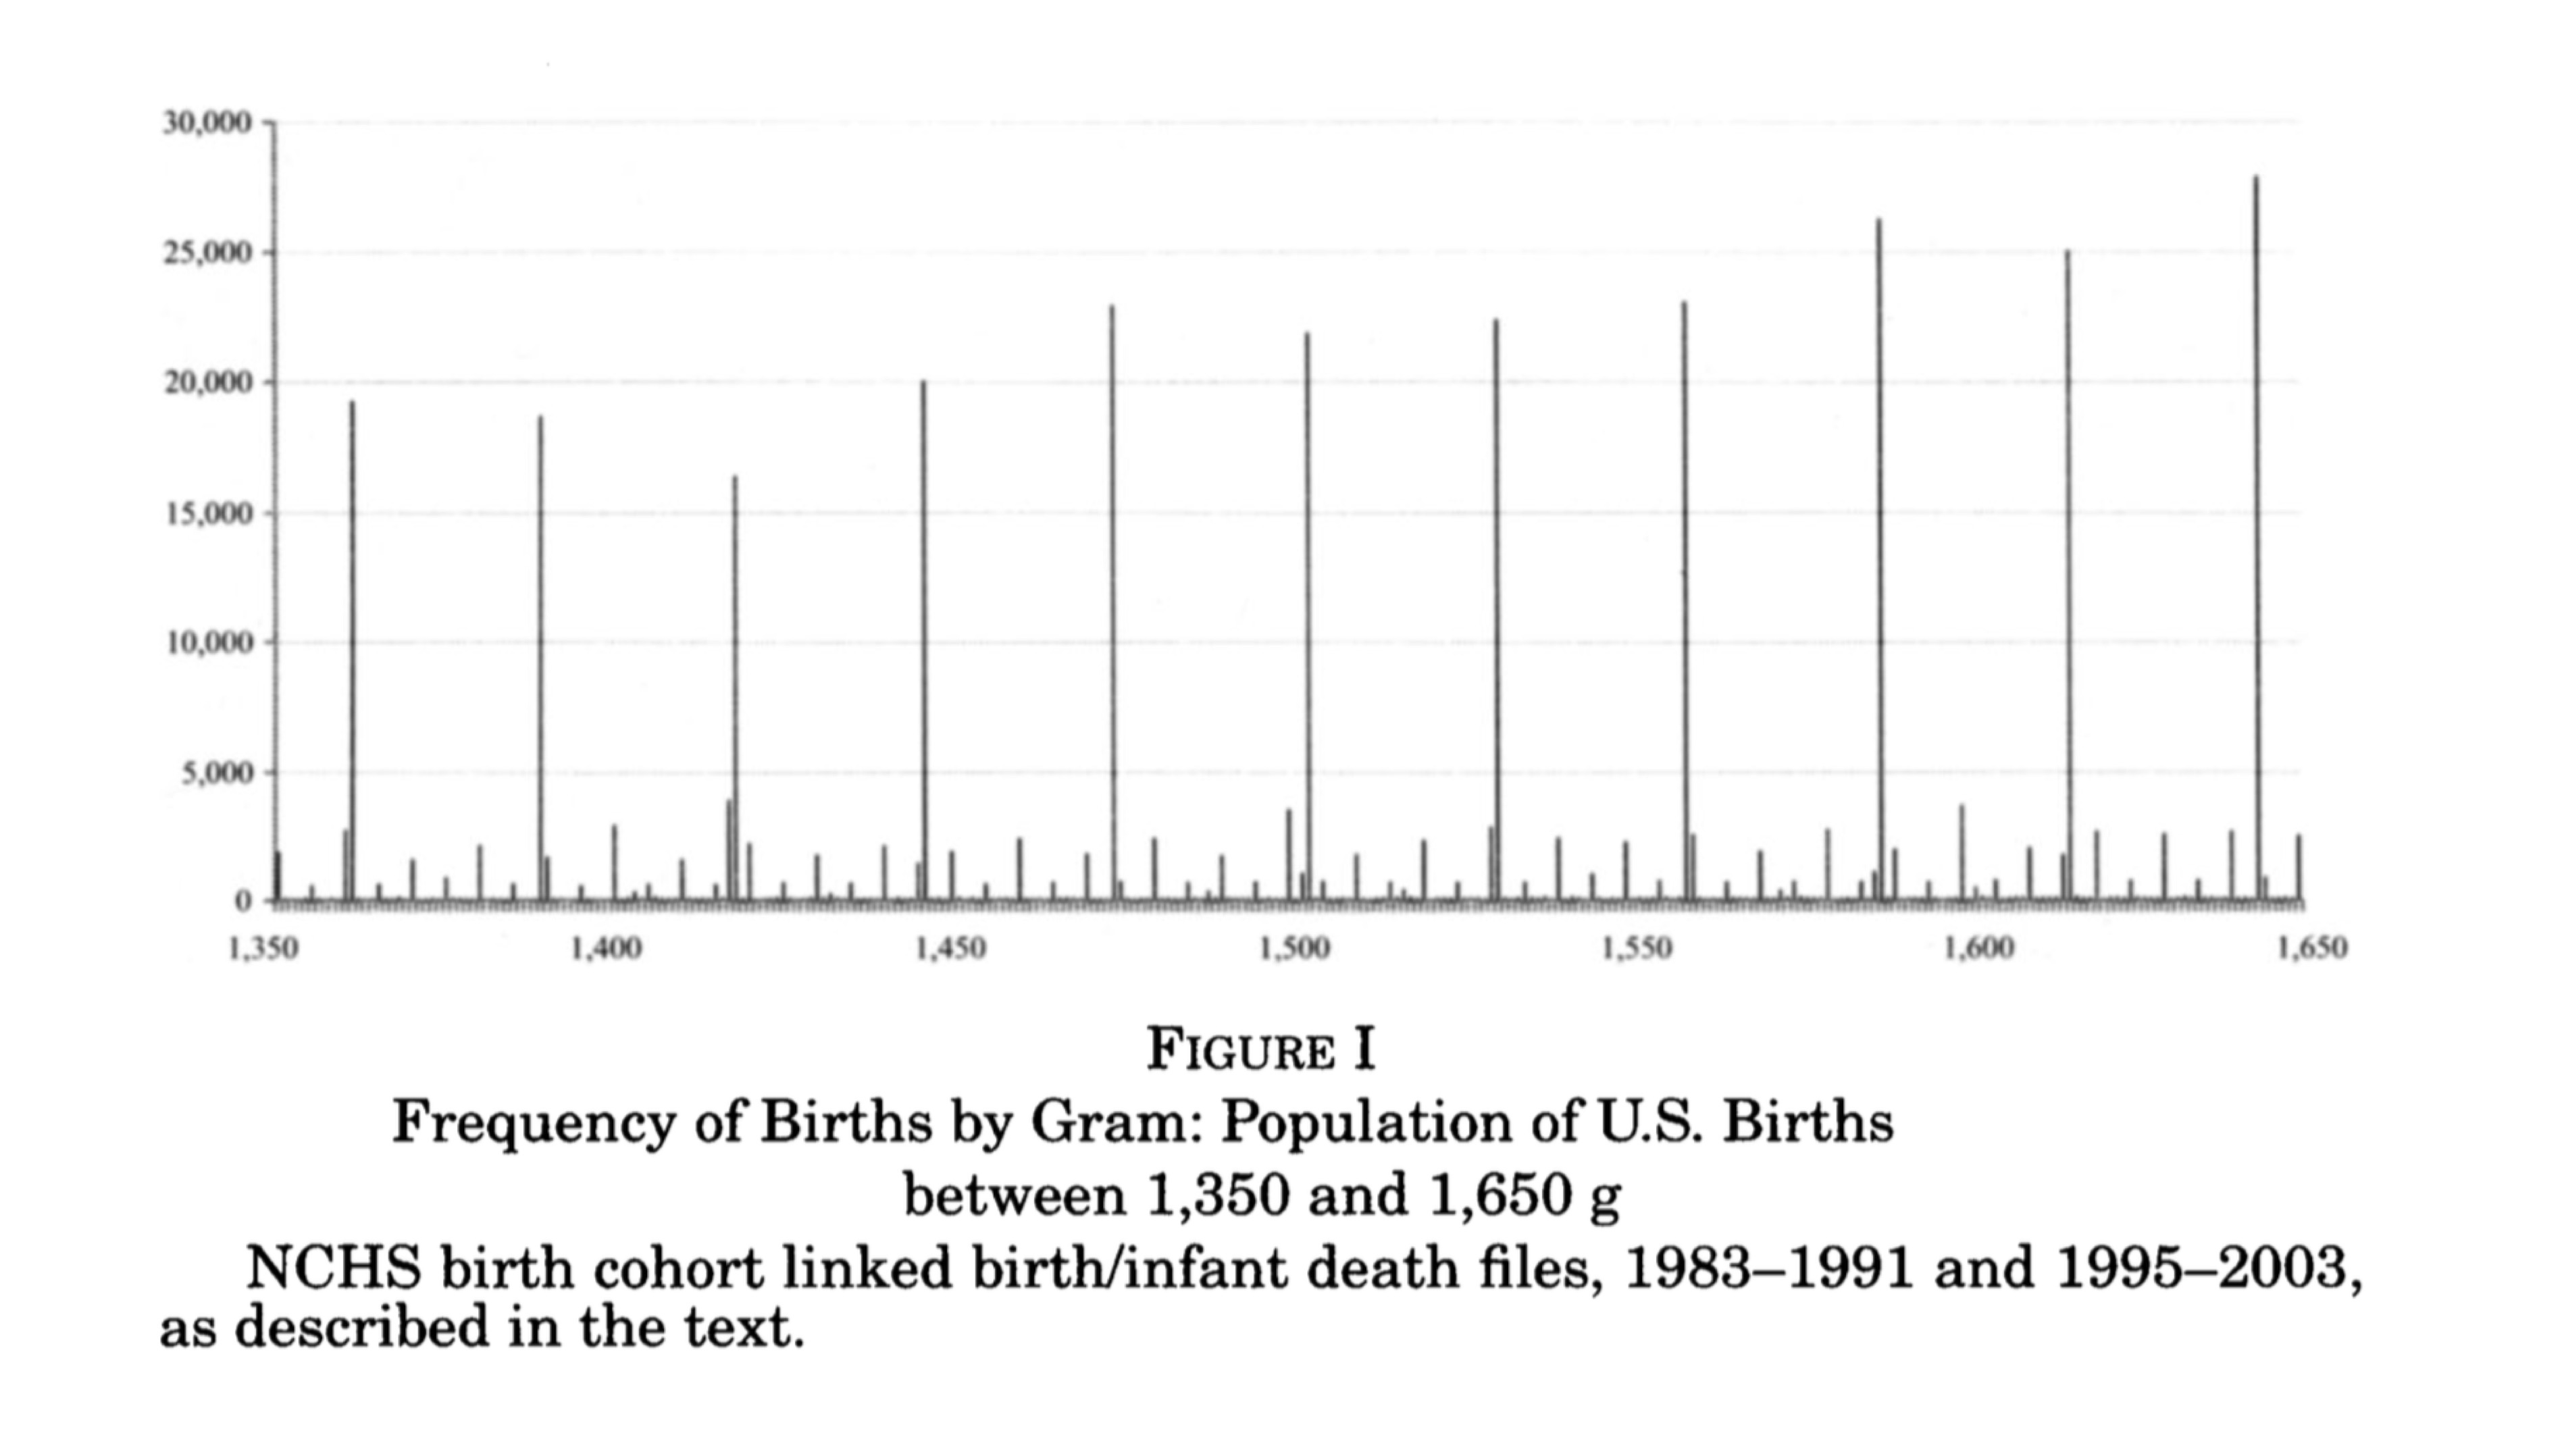
\includegraphics[scale=0.05]{img/heaping.jpg}
\end{figure}


\end{frame}

%%%%%%%%%%%%%%%%%%%%%%%%%%%%%%%%%%%%%%%%%%%%%%%%%%%%%%%%%%%%%%%%%%%%%%%%%%%%%%%%
\begin{frame}{Donut RDD}

Density tests cannot detect heaping, because of low power around the cut-off

\vspace{3ex}
Solution: Drop units in the vicinity of the cutoff and re-estimate the model
(called ``donut hole'')

\begin{itemize}
    \item Because of dropped units, the estimated parameter is an even more unusual local average treatment effect
    \item But this method allows for the possibility that units at the heap differ markedly due to selection bias
\end{itemize}

\end{frame}







\end{document}
